\documentclass[]{article}


%-----------------------------------------------------------------------------------------------------------------------------------------
%
%   GLOBALS
%
%-----------------------------------------------------------------------------------------------------------------------------------------
\newcommand{\DOCTITLE}{

}
\newcommand{\DOCAUTHOR}{

}
\newcommand{\DISCLAIMER}
{
    \topskip0pt
    \vspace*{\fill}
    {
    \centering
        \small{
            THIS DOCUMENT IS INTENDED FOR INTERNAL USE ONLY
        }
    }
    \\
    {
    \centering
        \small{
        UNAUTHORIZED DISTRIBUTION OF THIS DOCUMENT IS STRICTLY PROHIBITED 
        }
    }
    \vspace*{\fill}
}

\usepackage{lmodern}
\usepackage{amssymb,amsmath}
\usepackage{ifxetex,ifluatex}
\usepackage{fixltx2e} % provides \textsubscript
\ifnum 0\ifxetex 1\fi\ifluatex 1\fi=0 % if pdftex
  \usepackage[T1]{fontenc}
  \usepackage[utf8]{inputenc}
\else % if luatex or xelatex
  \ifxetex
    \usepackage{mathspec}
    \usepackage{xltxtra,xunicode}
  \else
    \usepackage{fontspec}
  \fi
  \defaultfontfeatures{Mapping=tex-text,Scale=MatchLowercase}
  \newcommand{\euro}{€}
\fi
% use upquote if available, for straight quotes in verbatim environments
\IfFileExists{upquote.sty}{\usepackage{upquote}}{}
% use microtype if available
\IfFileExists{microtype.sty}{%
\usepackage{microtype}
\UseMicrotypeSet[protrusion]{basicmath} % disable protrusion for tt fonts
}{}
\ifxetex
  \usepackage[setpagesize=false, % page size defined by xetex
              unicode=false, % unicode breaks when used with xetex
              xetex]{hyperref}
\else
  \usepackage[unicode=true]{hyperref}
\fi
\usepackage[usenames,dvipsnames]{color}
\hypersetup{breaklinks=true,
            bookmarks=true,
            pdfauthor={},
            pdftitle={},
            colorlinks=true,
            citecolor=blue,
            urlcolor=blue,
            linkcolor=magenta,
            pdfborder={0 0 0}}
\urlstyle{same}  % don't use monospace font for urls
\usepackage{longtable,booktabs}
\usepackage{graphicx,grffile}
\makeatletter
\def\maxwidth{\ifdim\Gin@nat@width>\linewidth\linewidth\else\Gin@nat@width\fi}
\def\maxheight{\ifdim\Gin@nat@height>\textheight\textheight\else\Gin@nat@height\fi}
\makeatother
% Scale images if necessary, so that they will not overflow the page
% margins by default, and it is still possible to overwrite the defaults
% using explicit options in \includegraphics[width, height, ...]{}
\setkeys{Gin}{width=\maxwidth,height=\maxheight,keepaspectratio}
\setlength{\parindent}{0pt}
\setlength{\parskip}{6pt plus 2pt minus 1pt}
\setlength{\emergencystretch}{3em}  % prevent overfull lines
\providecommand{\tightlist}{%
  \setlength{\itemsep}{0pt}\setlength{\parskip}{0pt}}
\setcounter{secnumdepth}{0}

\date{}

% Redefines (sub)paragraphs to behave more like sections
\ifx\paragraph\undefined\else
\let\oldparagraph\paragraph
\renewcommand{\paragraph}[1]{\oldparagraph{#1}\mbox{}}
\fi
\ifx\subparagraph\undefined\else
\let\oldsubparagraph\subparagraph
\renewcommand{\subparagraph}[1]{\oldsubparagraph{#1}\mbox{}}
\fi

%-----------------------------------------------------------------------------------------------------------------------------------------
%
%   PAGE SIZE AND MARGINS
%
%-----------------------------------------------------------------------------------------------------------------------------------------
\usepackage[a4paper,headheight=30pt]{geometry}
%\usepackage[letterpaper, portrait, margin=2in]{geometry}
\addtolength{\topmargin}{-.5in}
\addtolength{\textheight}{1.75in}

\usepackage{graphicx}

\usepackage{fancyhdr}
\pagestyle{fancy}


%-----------------------------------------------------------------------------------------------------------------------------------------
% Page break after sections
%-----------------------------------------------------------------------------------------------------------------------------------------
%\usepackage{titlesec}
%\newcommand{\sectionbreak}{\clearpage}

\lhead{
    %left header content
%    \topskip0pt
%    \vspace*{\fill}
    {
    \centering
        
\includegraphics[height=2.66em]{template/sc.png}
    }
%    \vspace*{\fill}
}
\chead{
    \topskip0pt
    \vspace*{\fill}
    {
    \centering
        \small{
            THIS DOCUMENT IS INTENDED FOR INTERNAL USE ONLY
        }
    }
    \\
    {
    \centering
        \small{
        UNAUTHORIZED DISTRIBUTION OF THIS DOCUMENT IS STRICTLY PROHIBITED 
        }
    }
    \vspace*{\fill}
}
\rhead{
%    \topskip0pt
%    \vspace*{\fill}
    % right header content
    {
    \centering
        
\includegraphics[height=3.25em]{template/scrd.png}
    }
%    \vspace*{\fill}
}
\lfoot{
    % left footer content
    \topskip0pt
    \vspace*{\fill}
    SCRD
    Revision 0.1
    \vspace*{\fill}
}
\cfoot{
    % middle footer content
    \topskip0pt
    \vspace*{\fill}
    {
    \centering
    SCRD Internal Documents Template \\
    \today
    }
    \vspace*{\fill}
}
\rfoot{
    % right footer content
    \topskip0pt
    \vspace*{\fill}
    \thepage
    \vspace*{\fill}
}
% extend the header into the margins
\usepackage{calc}
\fancyheadoffset[L,R]{\marginparsep+\marginparwidth}

%--------------------------------------------------------------------------------------------------------------
%	My Packages
%--------------------------------------------------------------------------------------------------------------
\usepackage{capt-of}

%--------------------------------------------------------------------------------------------------------------
%
%	BEGIN DOCUMENT
%
%--------------------------------------------------------------------------------------------------------------
\begin{document}


%--------------------------------------------------------------------------------------------------------------
%
%	TITLE PAGE
%
%--------------------------------------------------------------------------------------------------------------
\begin{titlepage}

\newcommand{\HRule}{\rule{\linewidth}{0.5mm}} % Defines a new command for the horizontal lines, change thickness here

\center % Center everything on the page
 
%----------------------------------------------------------------------------------------
%	HEADING SECTIONS
%----------------------------------------------------------------------------------------

\includegraphics[width=200pt,height=200pt]{../images/rocketry_logo_large.png}\\[1cm] % Include a department/university logo - this will require the graphicx package
\textsc{\Large Space Concordia - Rocketry Division}\\[0.5cm] % Major heading such as course name
\textsc{\large Aurelius CR-2-4G - Structural Team}\\[0.5cm] % Minor heading such as course title

%----------------------------------------------------------------------------------------
%	LOGO SECTION
%----------------------------------------------------------------------------------------

\begin{figure}[ht]
    \centering
    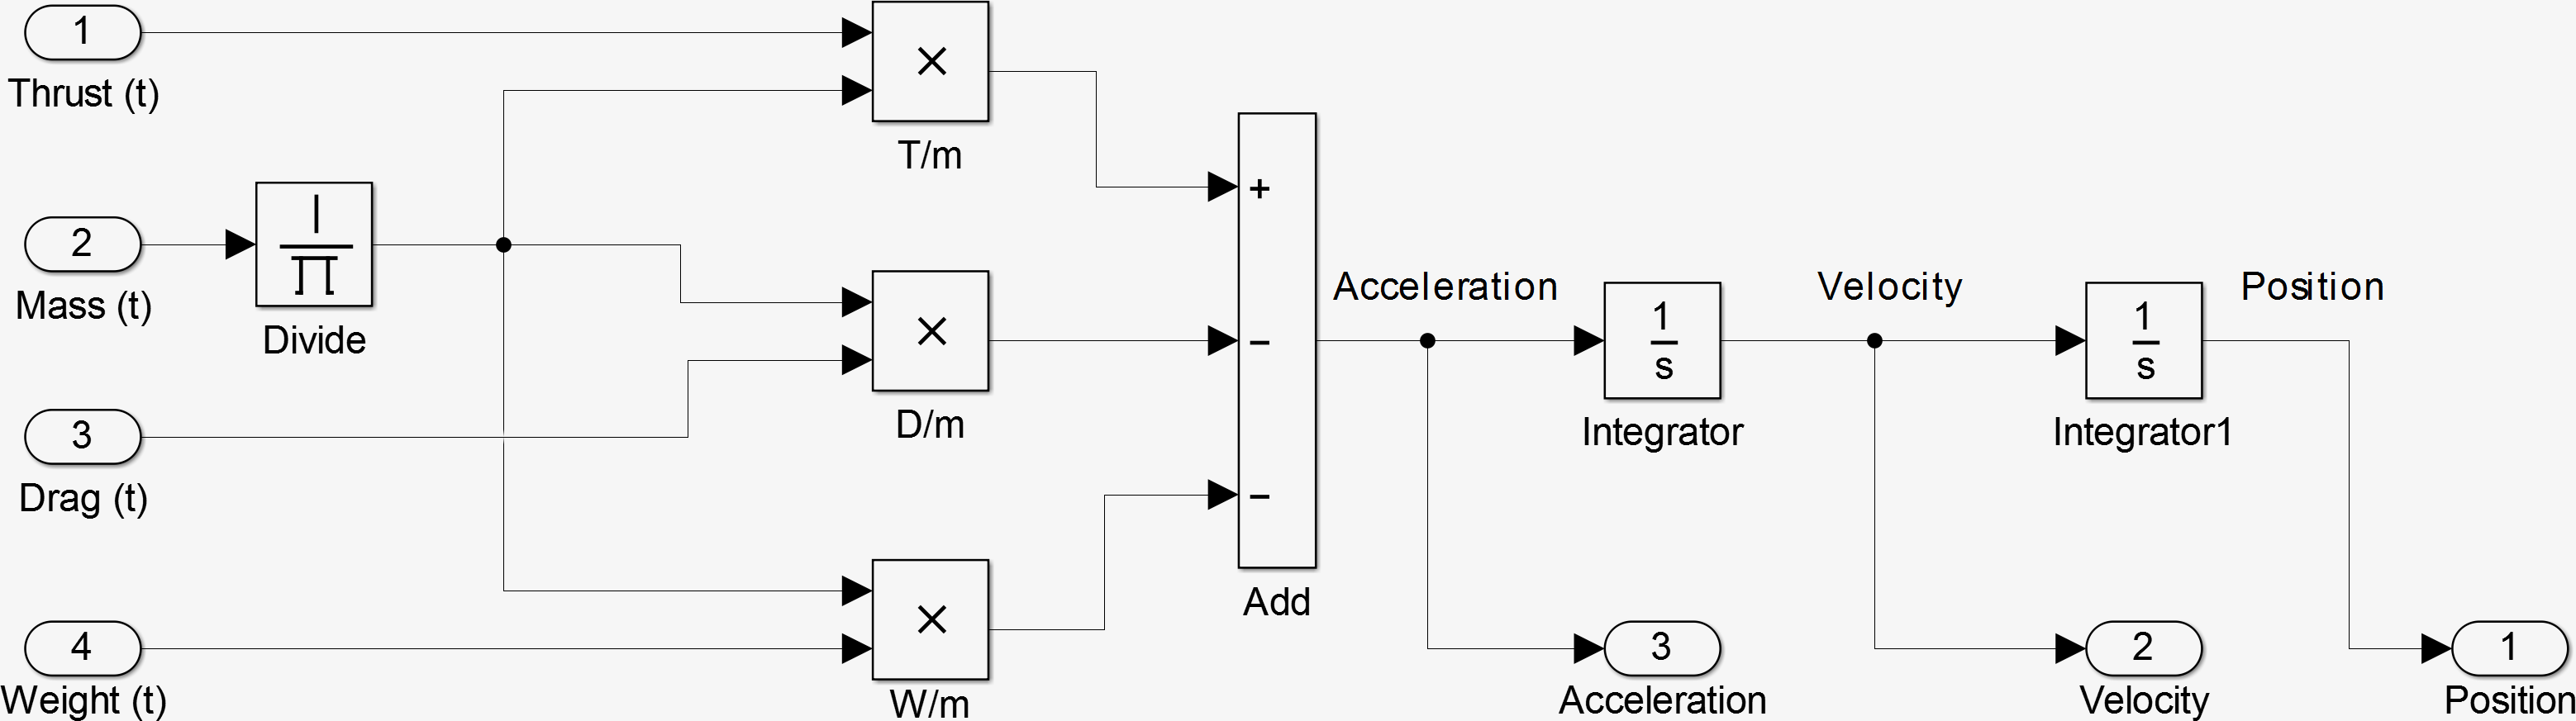
\includegraphics[height=100pt]{../images/vertical_model_simplified.png}\\
\end{figure}

%----------------------------------------------------------------------------------------
%	TITLE SECTION
%----------------------------------------------------------------------------------------

\HRule \\[0.6cm]
{ \Huge \bfseries 
Engineering Simulation for Rocket Flight Analysis
}\\[0.4cm] 

\HRule \\[1cm]
 
%----------------------------------------------------------------------------------------
%	AUTHOR SECTION
%----------------------------------------------------------------------------------------

\begin{minipage}{0.4\textwidth}
\begin{flushleft} \large
	\begin{tabular} {r l} 
        \emph{Author(s):} & Shawn Bulger	\\
	\end{tabular}
\end{flushleft}
\end{minipage}
~
\begin{minipage}{0.4\textwidth}
\begin{flushright} \large
	\begin{tabular} {r l} 
		\emph{Coordinator:} & Dr. Ashok Kaushal 		\\
		\emph{Supervisor:}  & Dr. Mehdi Hojjati 		\\
		\emph{EIR:}         & Dominic Ng  		        \\
	\end{tabular}
\end{flushright}
\end{minipage}\\[2cm]

%----------------------------------------------------------------------------------------
%	DATE SECTION
%----------------------------------------------------------------------------------------

{\large \today}\\[2cm] % Date, change the \today to a set date if you want to be precise

\vfill % Fill the rest of the page with whitespace

\end{titlepage}

{
\hypersetup{linkcolor=black}
\setcounter{tocdepth}{3}
\tableofcontents
\clearpage
}
\listoftables
\listoffigures
\clearpage
\section{Comparison with Experimental
Data}\label{comparison-with-experimental-data}

The University of Louisville was kind enough to share experimental
rocket flight data, as well as their rocket dimensions so that our
simulation could be compared to real-world experimental data.

\subsection{Flight Details}\label{flight-details}

\begin{longtable}[c]{@{}lllllll@{}}
\toprule
Date & Elevation & Ground Pressure & Ground Temperature & Wind Speed &
Humidity & Launch Guide Length\tabularnewline
\midrule
\endhead
20??/??/?? & 405 ft (123,48 m) & ?? Pa & ?? K (61.00 \(^\circ\)F) & ??
km/h (?? m/s) & ?? \% & 3.05 m (?? ft)\tabularnewline
20??/??/?? & 432 ft (131.71 m) & ?? Pa & ?? K (58.21 \(^\circ\)F) & ??
km/h (?? m/s) & ?? \% &\tabularnewline
20??/??/?? & 410 ft (125.00 m) & ?? Pa & ?? K (70.79 \(^\circ\)F) & ??
km/h (?? m/s) & ?? \% &\tabularnewline
20??/??/?? & 417 ft (127.13 m) & ?? Pa & ?? K (61.32 \(^\circ\)F) & ??
km/h (?? m/s) & ?? \% &\tabularnewline
20??/??/?? & 446 ft (135.97 m) & ?? Pa & ?? K (61.50 \(^\circ\)F) & ??
km/h (?? m/s) & ?? \% &\tabularnewline
\bottomrule
\end{longtable}

\subsection{Motor Details}\label{motor-details}

Cesaroni L935

\begin{longtable}[c]{@{}ll@{}}
\toprule
Parameter & Value\tabularnewline
\midrule
\endhead
Manufacturer: & Cesaroni Technology\tabularnewline
Entered: & Oct 6, 2009\tabularnewline
Last Updated: & Jun 26, 2014\tabularnewline
Mfr. Designation: & 3147L935-P\tabularnewline
Common Name: & L935\tabularnewline
Motor Type: & reload\tabularnewline
Diameter: & 54.0mm\tabularnewline
Length: & 64.9cm\tabularnewline
Total Weight: & 2542g\tabularnewline
Prop. Weight: & 1567g\tabularnewline
Cert. Org.: & Canadian Association of Rocketry\tabularnewline
Cert. Date: & Aug 27, 2009\tabularnewline
Average Thrust: & 933.8N\tabularnewline
Maximum Thrust: & 1585.6N\tabularnewline
Total impulse: & 3146.8Ns\tabularnewline
Burn Time: & 3.4s\tabularnewline
Isp: & 205s\tabularnewline
Case Info: & Pro54-6GXL\tabularnewline
Propellant Info: & Imax\tabularnewline
Data Sheet: & link\tabularnewline
Availability: & regularCesaroni L935\tabularnewline
\bottomrule
\end{longtable}

\subsection{Plots}\label{plots}

\begin{figure}[htbp]
\centering
\includegraphics{images/plot_experimental_comparison.png}
\caption{Plot of Simulation Data vs Louisville Rocket Launches
\label{experimental_comparison_label}}
\end{figure}

\hyperdef{}{refs}{\label{refs}}

\end{document}
